% !TEX encoding = UTF-8 Unicode
%!TEX root = thesis.tex

\newpage
\section{Background}

Prior to addressing the actual approach and implementation some concepts and terms have to be introduced. Firstly, the term \textit{security concept}, as it is used throughout the thesis, is being described. A definition of \textit{granularity levels} and system abstraction follows. Lastly, a section covers \textit{model transformations} and \textit{aggregation rules} on security attributes.

\subsection{Security}

Morrie Gasser \cite{Gasser} published a book in 1988 providing solutions for computer scpecialists interested in computer security. The term \textit{Computer Security} usually dealt with three aspects:

\begin{itemize}
\item Prevention of theft or damage to the hardware 
\item Prevention of theft or damage to the information
\item Prevention of service disruption
\end{itemize}

With the invention of the Internet the (personal) computers got interconnected and the sharing of data became prevalent and thus data security.

Nowadays security is seen as a process. No combination of products are guaranteed to make a system secure since they are only as secure as the people configuring them \cite{vacca2012computer}. \label{sec:security}

In general when talking about computer security three aspects are addressed, \textit{Confidentiality}, \textit{Integrity} and \textit{Availability} \cite{Pfleeger:2006:SC:1177321}. Each of them will no be defined:

\begin{itemize}
\item[] \textbf{Confidentiality} Assets can only be accessed by authorized parties
\item[] \textbf{Integrity} Assets can only be modified by authorized parties
\item[] \textbf{Availability} Assets are available to authorized parties when needed
\end{itemize} 

The challenge is seen in finding the right balance between the three \textit{Security Goals}. This situation is aggravated by the fact that the goals can overlap, be independent or even mutually exclusive. Charles P. Pfleeger \cite{Pfleeger:2006:SC:1177321} for example, addresses this problem by stating that a strong protection of confidentiality might restrict availability in a system.   

Information systems consist of hardware, software and data and it is of high importance for the respective stakeholder to secure the object of interest. When speaking about securing systems or components we look at two different terminologies, \textit{Vulnerabilities} and \textit{Threats}. A \textit{vulnerability} is a system weakness, be it in implementation or design, that can be potentially exploited by an adversary. Without the intent of exploiting it the vulnerability has no further effect on the system.

A \textit{threat} however is a set of circumstances that has the theoretical potential to cause harm by exploiting a specific vulnerability \cite{vacca2012computer}. An example to demonstrate the differences follows:

\begin{enumerate}
\item[] \textbf{Vulnerability}: Sending sensitive data over an unsecured channel \label{item:vuln}
\item[] \textbf{Threat}: Exploiting the unsecured channel by eavesdropping and gathering the sensitive data 
\end{enumerate}

As mentioned before a system weakness does not necessarily mean loss of data or any other system breach. Only when coupled with a set of circumstances and the intent of exploitation it turns into a threat. Figure \ref{fig:threats} illustrates the four acts that cause security harm as mentioned by Pfleeger \cite{Pfleeger:2006:SC:1177321}. 

\begin{figure}[H]
\centering
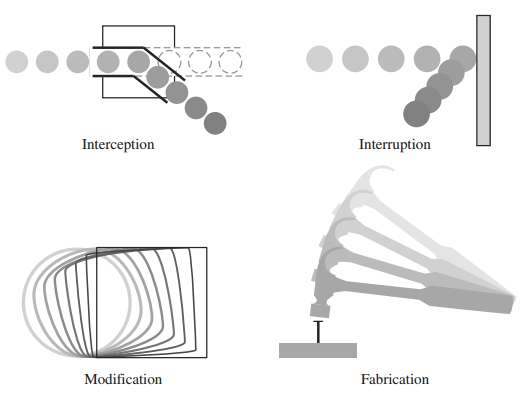
\includegraphics[width=0.85\textwidth]{pictures/threats.png}
\caption{Four acts that cause security harm}
\label{fig:threats}
\end{figure}

Confidentiality, integrity and availability, or the C-I-A triad like it is also being called, can be viewed from a perspective of the causes of harm. Confidentiality can suffer if some unauthorized party intercepts the data, availability can be lost if a flow of data is being interrupted and lastly integrity can be broken if the data is being modified or false data is being fabricated by an adversary.

To prevent the vulnerabilities from being exploited and the threats from potentially causing harm one can use \textit{Controls} or \textit{Countermeasures} to secure parts of a system. An example would be the use of encryption to prevent sensitive data from being eavesdropped on as mentioned in \ref{item:vuln}. 

To put everything into perspective the term \textit{Security Architecture} will be introduced.

\subsubsection{Security Architecture}

Gacek et al. discussed the definition of a \textit{Software System Architecture} (SSA) which will be used and adapted in the security context. According to the authors a \textit{Software System Architecture} is:

\begin{itemize}
\item A collection of software and system components, connections and constraints
\item A collection of system stakeholders' need statements
\item A rationale which demonstrates that the elements which define a system satisfy the the stakeholders' needs, if implemented correctly
\end{itemize}

Here, a \textit{Security Architecture} (SA) would be an adapted definition where, if implemented correctly, the stakerholders' \textit{security} needs will be satisfied. Naturally, the connections as well as the respective components might differ from the Software System Architecture as they might have to be enhanced or altered to satisfy the security needs. 

The stakeholders themselves however, are very similar. Gacek et al. differentiate between five parties, the \textit{Customer}, the \textit{User}, the \textit{Architect and System Engineer}, the \textit{Developer} and the \textit{Maintainer}. 

The International Standard ISO 27001 provides a model for establishing, impelementing, operating, monitoring, reviewing, maintaining and improving an organization's Information Security Management System \cite{iso27001}, i.e. a system that is responsible for establishing and maintaining organization's security needs and guidelines. When comparing these rather short definitions one can already see an overlap when looking at potential stakeholders. An overview on the SSA stakeholders follows:

\begin{tabular}{|c|c|}
\hline
Stakeholder & SSA Concern \\
\hline
Customer & \makecell{Schedule and budget estimation \\ Feasibility and risk assessment \\ Requirements traceability \\ Progress tracking} \\
\hline
User & \makecell{Consistency with requirements and usage scenarios \\ Future requirement growth accommodation \\ Performance, reliability, interoperability} \\
\hline
\makecell{Architect and \\ System Engineer} & \makecell{Requirements traceability \\ Support of tradeoff analyses \\ Completeness, consistency of architecture} \\
\hline
Developer & \makecell{Sufficient detail for design \\ Reference for selecting/assembling components \\ Maintain interoperability with existing systems} \\
\hline
Maintainer & \makecell{Guidance on software modification \\ Guidance on architecture evolution \\ Maintain interoperability with existing systems} \\
\hline
\end{tabular}      
\vspace{3mm}

When looking into the International Standard, one can see that similar concerns can be also found in the adaptation of the \glqq Plan-Do-Check-Act\grqq \ model for the establishment of an ISMS process. In the case of ISMS similar aspects can be found in the four different phases as seen in Figure \ref{fig:isms_stakeholder}. 

\begin{figure}[H]
\centering
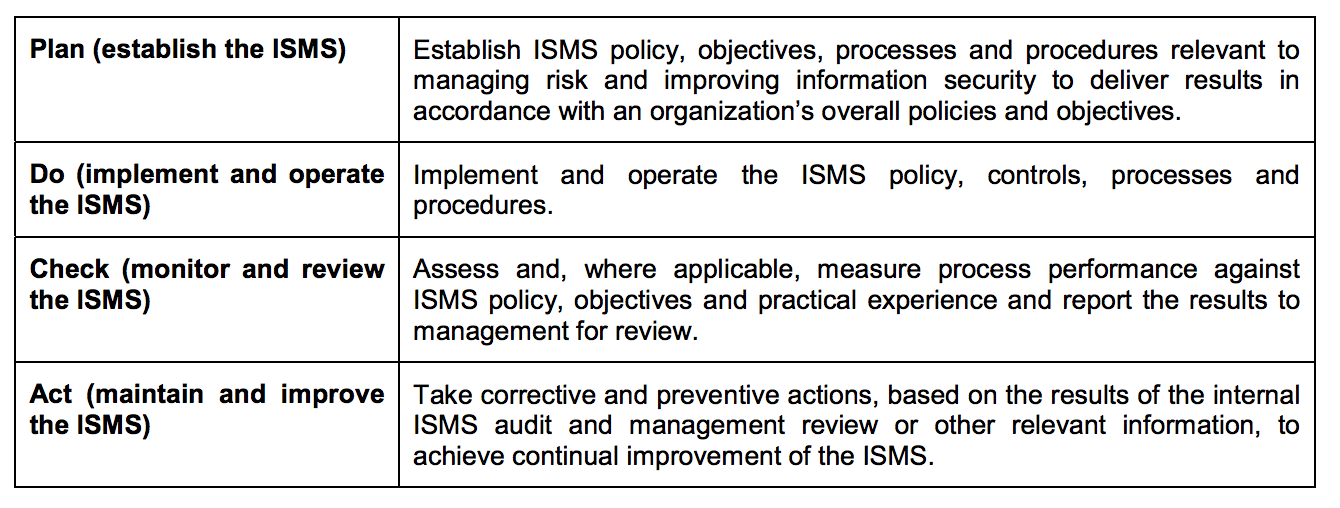
\includegraphics[width=\textwidth]{pictures/isms_concerns.png}
\caption{ISMS Stakeholder Concerns}
\label{fig:isms_stakeholder}
\end{figure}

Security requirements and objectives have to be defined in the earlier phases so they can be planned, implemented and carried out by the respective security architects/developers/security engineers. Here, the term user is not as clear since a variety of employees can be seen as such, e.g. any employee that accepts the established security policies. Since systems, as mentioned in Section \ref{sec:security}, are just as secure as the people using them, many employees can be viewed as ISMS users. They would be interested in implementing and operating the processes and procedures which have been defined in the previous phase.

Established security policies have to be also monitored and maintained. Security is never guaranteed and is a complex process \cite{vacca2012computer} - systems have to be constantly updated and possibly upgraded. 

A Security Architecture is therefore a union of security objectives by different stakeholders and, if properly implemented, guaranteees the stakeholders' needs.
These needs have to be considered throughout the system processes and have to be registered in a comprehensible manner. Security requirements have been mentioned and, amongst others, will be described more thoroughly in the next section.

%\subsection{Enterprise Security}
%To define the term \textit{security concept} one has to look at the architecture of enterprises to understand the interconnectivity and interdependence between services, security being one of them. 
%
%\subsubsection{Enterprise Architecture}
%
%Information systems tend to be a very complex artifacts that combine different views and requirements from various stakeholders of different backgrounds \cite{alex}. 
%
%Software, IT platforms and IT related goals in general are covered in an \textit{Information System Architecture} (ISA). ISA does not take any business-driven influences into account and is therefore insufficient when describing the complex dependencies in corporations, especially when it comes to security as described in Subsection \ref{subsec:secarch}.   
%
%\textit{Enterprise Architecture Modeling} tries to overcome such possible difficulties and combines IT related concerns with business and organizational goals and shows possible interrelationships. It therefore provides an approach for an improved understanding of complex enterprise processes \cite{earch}. The Federal Deposit Insurance Corporation (FDIC) published the results of an audit of its own implementation of E-Government principles \cite{fdicaudit} and their division of information technology in Figure \ref{fig:fdic} depicts the interrelations very well. 
%
%\begin{figure}[H]
%\centering
%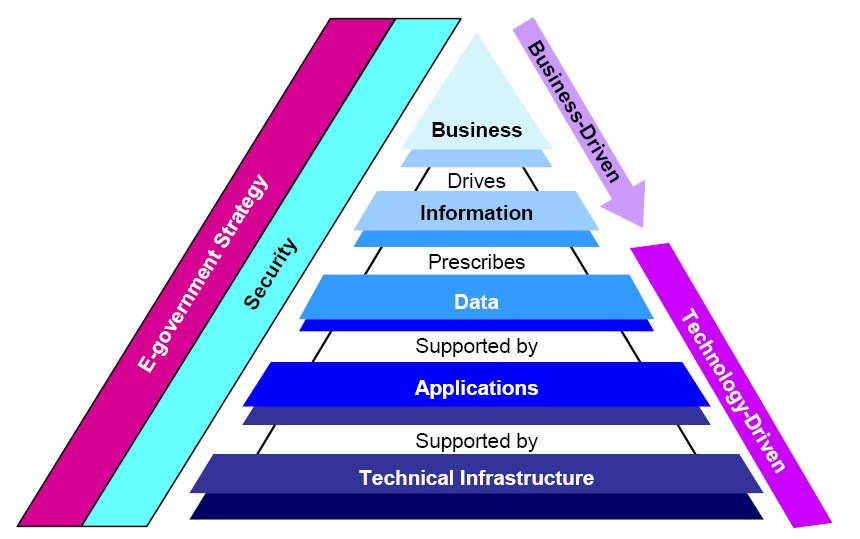
\includegraphics[width=0.75\textwidth]{pictures/fdic.jpg}
%\caption{Division of Information Technology by FDIC}
%\label{fig:fdic}
%\end{figure}
%
%\subsubsection{Security Architecture}
%\label{subsec:secarch}
%
%Information Security has often been merely an afterthought in corporations \cite{ansfederal} until a concept of a \textit{Security Architecture}, published in a whitepaper by The Gartner Group \cite{kreizman}, was introduced. According to \cite{kreizman} an \textit{Enterprise Information Security Architecture} (EISA) is an essential tool for improving security processes in corporations. EISA principles stand in a direct relationship with the EA principles and should be validated against them \cite{kreizman}. To highlight this relationship security considerations during phases of the \textit{The Open Group Architecture Framework Architecture Development Method} (TOGAF ADM), which is shown in Figure \ref{fig:togaf}, will be briefly described.
%
%\begin{figure}[H]
%\centering
%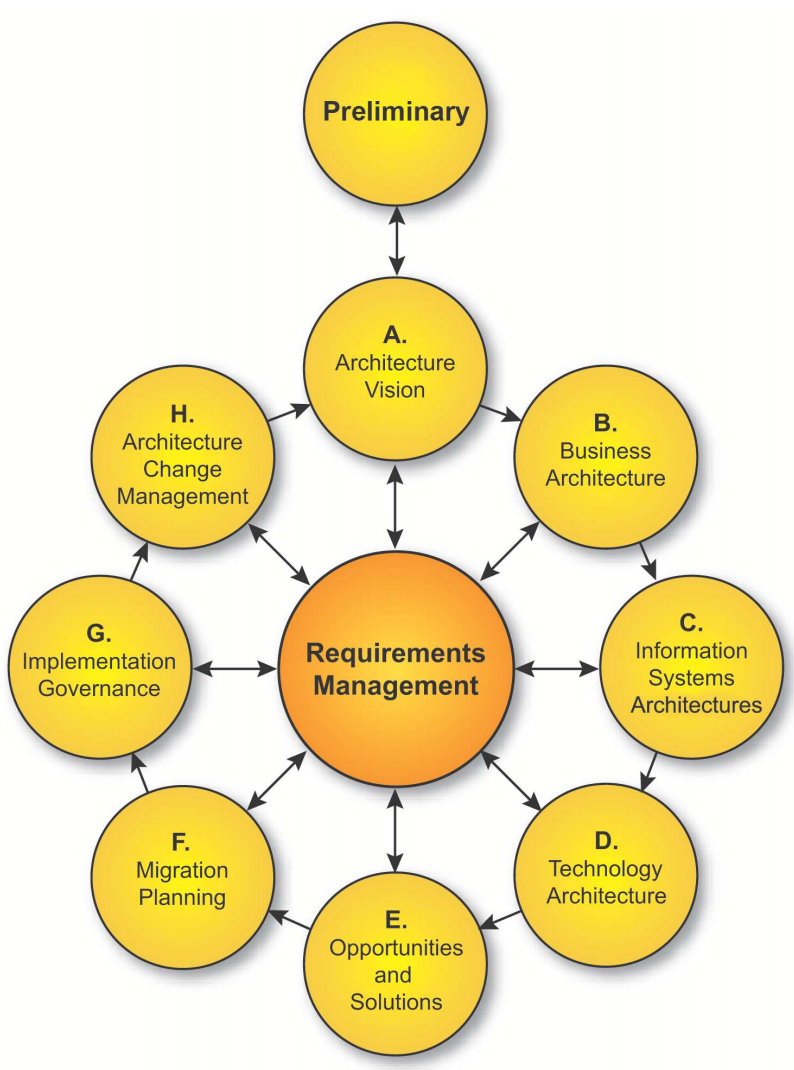
\includegraphics[width=0.6\textwidth]{pictures/togaf_overview.png}
%\caption{Overview of the phases of TOGAF}
%\label{fig:togaf}
%\end{figure}
%
%Security concerns can be found throughout the TOGAF phases which hints at the overall importance of security in corporations. TOGAF combines four architecture domains, the \textit{Business Architecture}, the \textit{Data Architecture}, the \textit{Application Architecture} and the \textit{Technology Architecture}. The following section will depict security considerations of two domains to show possible interrelations.
%
%During the \textit{Business Architecture} phase in the ADM actors and handlers of the system have to be identified. Costs and potential incoveniences because of security measures have to be assessed as well. In general one can say that the impacts of security/insecurity on the business/product are being highlighted. It is tried to put an emphasis on security as early as possible to prevent costly changes in later phases in the ADM.
%
%During the \textit{Information System Architecture} phase the classification levels of processed data have to be determined and documented. Direct dependencies to the \textit{Business Architecture} are also listed, e.g. the identification of information lifespan according to business goals and regulations. 
%
%Similar relations can be found for security considerations from various phases of the ADM. This once again shows the overall presence of security and the high level of complexity within an enterprise.

\subsubsection{Common Criteria}
The following section will present a way of modeling security concerns for an asset of interest.

Common Criteria proposes an evaluation by using a so called \textit{Security Target} (ST), a construct that encapsulates the \textit{Target of Evaluation} (TOE), threats to the TOE and countermeasures \cite{commoncriteria}. The goal of the evaluation is to show that the used countermeasures are sufficient to counter potential threats and thus implying that the TOE is sufficiently protected.

\begin{figure}[H]
\centering
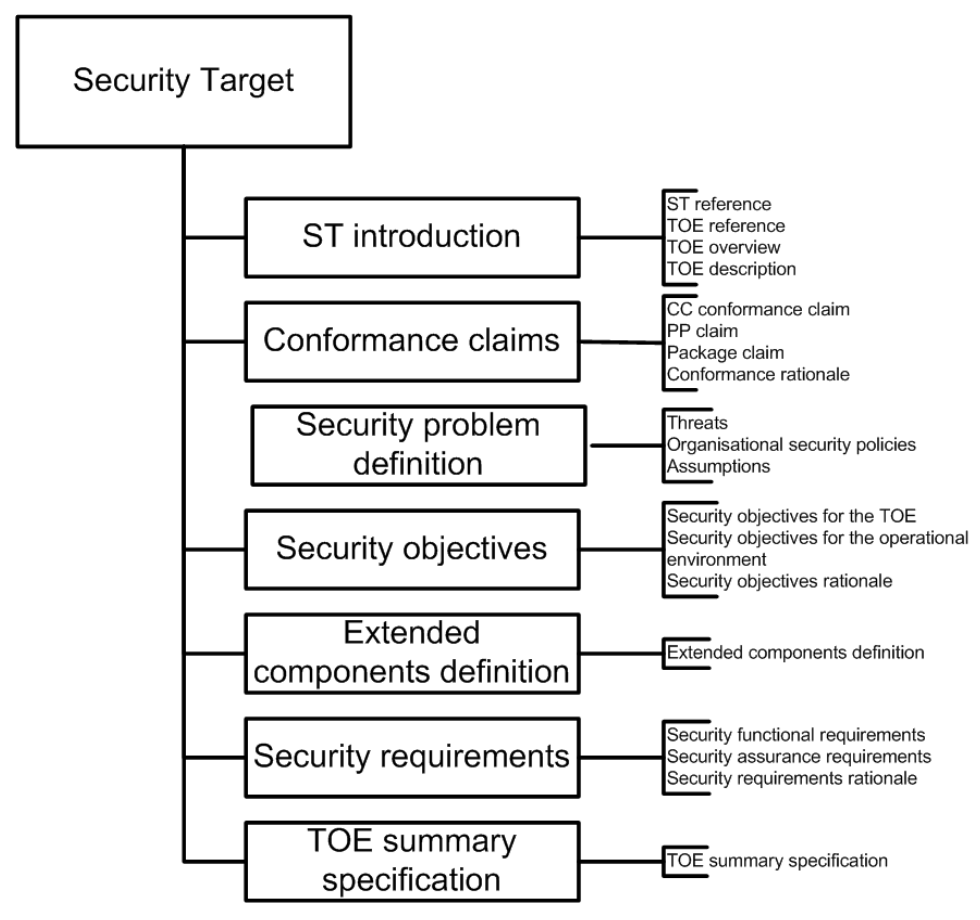
\includegraphics[width=0.85\textwidth]{pictures/sectarget.png}
\caption{Overview of the Security Target contents}
\label{fig:sectarget}
\end{figure}

A description of all the contents of a ST is unnecessary here and only the key security attributes of a ST that will be used to construct a \textit{Security Concept} (Subsection \ref{subsubsec:secconc}) are being introduced.

The \textit{Security Problem Definition} defines, as the name suggests, the security problem that is being addressed. Apart from containing guidelines and assumptions it contains \textit{Threats} which are \textit{\glqq[...] adverse actions performed by a threat agent on an asset\grqq} (\cite{iso27001}, p. 66).

A \textit{Security Objective} is an abstract solution to the previously defined security problem. There exists a possibility to divide the \textit{Security Objectives} into part wise solutions, one being the \textit{Security Objectives for the TOE} and the other being the \textit{Security Objectives for the Operational Environment}. Moreover does the ST contain traces showing which objectives address which threats, guidelines and assumptions and a set showing that all threats, guidelines and assumptions are addressed by the security objective.

\textit{Security Functional Requirements} (SFR) are a more detailed translation of the previously defined \textit{Security Objective}. Despite being more detailed, SFR have to be still independent from specific technical solutions. 

Lastly, STs contain a TOE summary specification where it is stated how the TOE meets all the SFRs and how exactly those requirements are met on a technical level.

\subsubsection{Security Concept}
\label{subsubsec:secconc}

The term \textit{Security Concept}, as it is defined here, is based on the constructs introduced in the previous chapters, namely \textit{Security Architecture} and \textit{Security Target}. An overview follows. 

\textit{Assets} are the to be secured objects of interest, i.e. TOE according to Common Criteria. \textit{Assets} can be either logical or physical and can be grouped to sets, if needed.

A \textit{Security Goal} (SG) is the equivalent to the \textit{Security Objective}. A valid SG must address an \textit{Asset} and a \textit{Security Goal Class} that defines the actual purpose of the SG. In general the set of \textit{Security Goal Classes} consists of \textit{Confidentiality}, \textit{Integrity} and \textit{Availability} but can also be expanded by further classes such as \textit{Authenticity}.

\textit{Threats} serve the same purpose as proposed by Common Criteria. They are adverse actions performed by an entity against an \textit{Asset}. 

This information is all brought together in \textit{Security Requirements} that are defined in natural language and show the interrelationships between elements. A \textit{Security Goal} has to be mentioned as well as an \textit{Asset} and a \textit{Threat} against which the object of interest should be protected.

Lastly, \textit{Controls} are the technical measures that counter or minimize the \textit{Threats}.     

The Table \ref{table:secconc} depicts the relationships between all the security attributes:

\begin{sidewaystable}
\begin{tabular}{|c|c|c|c|}
\hline
\textbf{Name} & \textbf{Contains} & \textbf{Description} & \textbf{Example} \\
\hline
\multirowcell{3}{Asset} & \multirowcell{3}{-} & \multirowcell{3}{Digital or physical object of \\ interest \\ that should be secured} & \multirowcell{3}{Sensible user data} \\
& & & \\
& & & \\
\hline
\multirow{2}{*}{Security Goal Class} & \multirow{2}{*}{-} & \multirowcell{2}{Defines the purpose \\ of the Security Goal} & \multirowcell{2}{Confidentiality of sensible \\ user  data} \\
& & & \\
\hline
\multirow{2}{*}{Security Goal} & \multirow{2}{*}{Security Goal Class, Asset} & \multirowcell{2}{Defines the security \\ objective} & \multirowcell{2}{ Confidentiality of sensible \\ user data shall be protected} \\
& & & \\
\hline
\multirow{2}{*}{Threat} & \multirow{2}{*}{Asset} & \multirowcell{2}{Adverse action against an \\ Asset} & \multirowcell{2}{Eavesdropping on sensible \\ user data} \\
& & & \\
\hline
\multirowcell{4}{Security Requirement} & \multirowcell{4}{Asset, Security Goal, Threat} & \multirowcell{4}{Security Objective \\ in natural language} & \multirowcell{4}{
The Confidentiality of \\ sensible user data shall \\ be protected against \\ eavesdropping} \\
& & & \\
& & & \\
& & & \\
\hline
\multirowcell{3}{Control} & \multirowcell{3}{Threat} & \multirowcell{3}{Measure to minimize \\ or mitigate the Threat} & \multirowcell{3}{Encryption of sensible user \\ data with AES-256 \\ to prevent eavesdropping} \\
& & & \\
& & & \\

\hline
\end{tabular}
\caption{Elements of a Security Concept}
\label{table:secconc}
\end{sidewaystable}

\subsection{Modeling}
\label{subsec:interpretation}
To ensure a viable solution one has to think of a representation of real life systems. \textit{Models} can be used to achieve this by depicting the key properties and processes of a certain system. According to Ed Seidewitz \cite{seidewitz} a model is a \textit{\glqq set of statements about some system under study\grqq} with the statements being either correct or incorrect.

A system modeled using the Unified Modeling Language (UML) serves as an example. In this case such statements could be made on the relationships between classes and would only be correct if they are consistent with the actual structure of the respective system under study (SUS), i.e. the described (modeled) relationships do indeed exist. 

In our case we would try to create a model that reflects the security attributes and their interrelationships in a SUS. This interpretation of a model is key because only then the model is given a meaning \cite{seidewitz}.

A definition of a model is not enough. A \textit{metamodel} has to be clearly defined to verify whether a model is conform or not, i.e. whether a security concept instance is conform to its security concept metamodel. The following figure shows the interrelationships.

\begin{figure}[H]
\centering
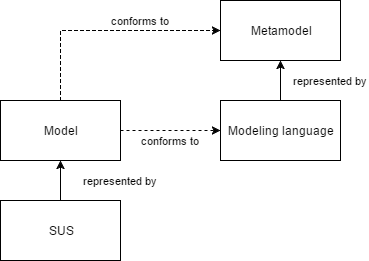
\includegraphics[width=0.75\textwidth]{pictures/metamodel.png}
\caption{Relationships between Model and Metamodel}
\label{fig:metamodel}
\end{figure}

A security concept of a SUS would be modeled in a modeling language, e.g. UML which is a representation of its own metamodel. At the same time the security concept would be conform to its metamodel. This conformity, be it the security concept or the modeling language, is needed for a model to be considered valid. 

\subsubsection{Model Transformation}
\label{subsubsec:modeltrans}
The Meta Object Facility (MOF) \cite{omg2013mof} is a standard metametamodel proposed by the Object Management Group (OMG) and captures the relationships between models in a three-layered architecture consisting of M1, M2 and M3. Models (M1) are representations of systems and are expressed in a modeling language M2, e.g. UML as mentioned in the previous section, which is conform to a so called metamodel. Metamodels themselves are also expressed in a metamodeling language which is conform to a metametamodel (M3). 

These architecture levels can be found in the \textit{model transformation pattern} by Jouault et al. \cite{modeltrans} which can be seen in Figure \ref{fig:metametamodel}. 

\begin{figure}[H]
\centering
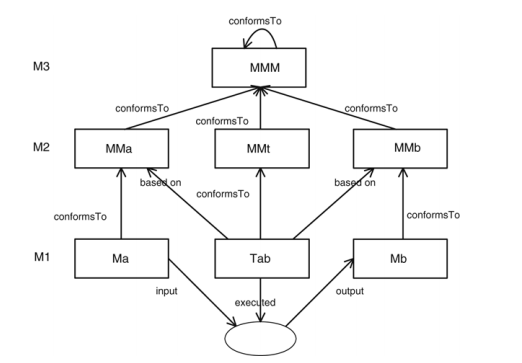
\includegraphics[width=\textwidth]{pictures/metametamodel.png}
\caption{Model transformation according to Jouault et al.}
\label{fig:metametamodel}
\end{figure}

Here a source model $Ma$ is being transformed into a target model $Mb$ using a transformation language. Both models and the transformation language are conform to their respective metamodel which is the traditional understanding of a model transformation.

Kleppe et al. defined a \textit{transformation} as an automatic generation of a target model from a source model according to \textit{transformation rules} that describe how elements from the source model can be transformed into a target model \cite{Kleppe:2003:MEM:829557}. 

This transformation may have different levels of automation. An \textit{automatic} transformation would not need any manual intervention from the user. In cases where incompleteness or inconsistencies may occur a manual intervention may be needed \cite{mt_taxonomy}.

Throughout the introduction and the background chapter the derivation of security attributes based on structural properties of a system of interest was mentioned. Given a model $M$ this derivation can be seen as alteration of $M$ and therefore as a \textit{model transformation}. The resulting model $M'$ is different to $M$, both however, are conform to the same metamodel $MM$ whereas $MM$ is conform to $MMM$. In our case both source and target languages are identicial. We can therefore simplify the transformation graph shown in Figure \ref{fig:metametamodel}.

\begin{figure}[H]
\centering
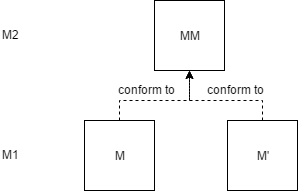
\includegraphics[width=0.55\textwidth]{pictures/transformation.png}
\caption{Model transformation}
\label{fig:transformation}
\end{figure}

The definition of a transformation $T$, or better a \textit{transformation rule set}, that alters a model $M$ is the main goal of this thesis.

Prior to the actual rule set definition one final concept has to be introduced. A user-selected \textit{Granularity level} serves as a second input in the model transformation. The transformation itself should be automatic, the only user input should be the just mentioned granularity level.

\subsubsection{Granularity Levels}
\label{subsubsec:granularity}

Information systems are often complex because of the number of interconnections and interdependencies between components and therefore it might be difficult to assess potential impacts and risks of a system \cite{branagan}.

One logical goal would be to decrease the overall complexity to enable a better risk assessment. \textit{System abstraction} tries to achieve this by reducing the level of details \cite{branagan}. Thyssen et al. differentiate between two possibilities, \textit{Whole-part decomposition} which decomposes a system into smaller sub-systems and \textit{Distinct development perspectives} which focuses on certain parts of a system depending on the current development perspective. 

In this thesis the focus will be on the \textit{Whole-part decomposition} even though an adaption of development perspectives is certainly possible. The main difficulty would be the definition of such perspectives in the security context because they would be highly dependent on the respective security analyst. The perspectives would not be unambiguous.
  
Therefore the change of the level of detail, i.e. the granularity level, will be achieved by uniting or decomposing components of a system of interest. By decomposing a larger system into smaller sub-systems one could focus on only specific security attributes and dismiss others.

A user will select a certain granularity level, i.e. a certain set of components, as an input to the transformation function $T$ as mentioned in \ref{subsubsec:modeltrans}. Together with the defined rule set a valid model $M'$ will be generated which to be considered valid has to be conform to its metamodel $MM$.

\section{Related Work}
\label{sec:related_work}

Several publications that provide an essential basis for this thesis will now be presented. A variety of different topics will be briefly covered such as abstraction layers/granularity layers, security attribute aggregation and propagation as well as model transformations and formal verification. 

\subsection{Granularity layers}

Thyssen et al. presented a framework which allowed them to view models under different levels of abstraction \cite{thyssen2010system}. This abstraction is achieved by introducing granularity levels which are based on the different needs of the stakeholders. 

Two different approaches were suggested where one is \textit{Whole-part decomposition} which applies the divide-and-conquer principle and decomposes the SUS into smaller blocks until atomic blocks are reached. The other possible method is viewing the system from \textit{Distinct development perspectives}. The differences have already been briefly discussed in Section \ref{subsubsec:granularity} and therefore only whole-part decomposition will be presented in more detail. 

Thyssen et al. propose a decomposition of systems into sub-systems to overcome the complexity. A sub-system is seen as a independent system by itself and the goal is to achieve \glqq seamless\grqq \ abstraction. This way the sub-systems could be viewed separately and, if needed, could be aggregated to the overall system.

Different development perspectives were also proposed to focus on specific stakeholders and their needs during the system abstraction. 

The \textit{user perspective} describes, as the name suggests, the user's interests and the fulfilment of such by the respective system. The focus is on the hierarchical structuring of the general system functionality based on the users' needs and the functional interrelationships between components. The \textit{logical perspective} can be seen as a bridge between the user-defined requirements and the technical implementation and lastly, the \textit{technical perspective} describes the technical side, i.e. the hardware components that incorporate the needs of the respective users.  

In this thesis however, the main focus is the combination of the security perspective and the \glqq seamless\grqq \ abstraction of systems. As previously mentioned security in information systems is seen as a complex process \cite{vacca2012computer} and the realization of security policies may have effects on different perspectives. Throughout the thesis system abstraction will be addressed from the perspective of a security architect that tries to incorporate all the stakeholders' security needs in a system. The goal is to propose a solution on how security properties of systems propagate through different levels of abstraction. Dependencies amongst them have to be taken into account and appropriate aggregation rules have to be defined. 

Thyssen et al. have introduced the theoretical idea of \glqq seamless\grqq \ abstraction but have not addressed the the transformation steps that are needed to transform a system from one granularity level to another.  

\subsection{Security Attribute Aggregation}

Aggregation of security attributes has been studied and aggregation rules have been discussed by multiple researchers. Menzel et al. focused on the aggregation of security requirements and dependencies amongst them \cite{Menzel2008}. They defined interaction sets for requirements that classified the effects two requirements $r_1$ and $r_2$ might have on each other. According to \cite{Menzel2008} requirements could be independent, equivalent or conflicting, just to name a few.

Furthermore, when addressing the actual aggregation, Menzel et al. argued that to propose correct rules one has to look at two core aspects. Firstly one has to determine whether two requirements belong to the same class of security goals or not and secondly, the addressed entities and dependencies amongst the requirements have to be considered.

The transformation rules, which will be defined in Section \ref{sec:approach}, use this concept as the basis. Even though Menzel et al. have not addressed the needed transformation steps they provided core aspects that are essential for the aggregation of requirements. These will also be considered during application for different security attributes.

Similarities can be found when looking at the work carried out by Noel et al. \cite{Noel:2004:MAG:1029208.1029225} which addresses attack graph aggregation. 

Attack graphs are a representation of possible vulnerabilities in a network that can be exploited by attackers.  Interactions and dependencies are represented by edges and for large networks such graphs may become very complex. To reduce the just mentioned complexity rules have been introduced that hierarchically aggregate graph elements. 

Rules for exploits and security conditions, i.e. states that exist prior to or after an exploit, have been proposed. Exploits are being aggregated based on the attacker/victim machines where only exploits on the same machines are being aggregated into exploit sets. 

Conditions are being aggregated into condition sets when they are either preconditions or postconditions of the same exploit. Later on, an aggregation based on machine level is being executed, i.e. conditions are being aggregated if they all occur on the respective machine. A machine is therefore a union of all its conditions. 

Both the idea of aggregation based on same elements/machines as well as the idea of union sets consisting of conditions will be adapted in this thesis.

Lastly, risk aggregation is being covered. Lenstra et al. \cite{Lenstra2004}  have discussed both the qualitative as well as the quantitative risk analysis providing both the advantages and disadvantages of the respective method. Qualitative risk analysis assigns subjective values to risks or threats (such as High, Medium or Low) and these values then display the severity of the respective threat or risk. Qualitative approaches however, only provide very vague indications which might not be suitable for specific, more complex systems. 

Quantitative approaches view the underlying events as distribution functions and derive the overall risk of an element from said functions. As mentioned by Lestra et al. and example could be the \textit{Annual Loss Expectancy} for an event which can then be aggregated when viewing different events.

In our case quantitative aggregation is not necessary and might not even be possible in many cases since the given security concepts might be underspecified. 

Our goal is to provide a solution on security attribute propagation for as many systems as possible applying qualitative aggregation for security attributes defined in the metamodel in Section \ref{subsec:sec_concept}. Although it is less precise than quantitative approaches \cite{Lenstra2004} it suffices when considering the possibility of underspecification of security concepts and the overhead during aggregation steps when applying such an analysis.

\subsection{Validation of Model Transformations}

When proposing the model transformation one has to determine its correctness. Varro et al. define four properties that verify the correctness of a model transformation \cite{vacca2012computer}.

\begin{itemize}
\item[]\textbf{Syntactic correctness:} The generated model is a syntactically correct model instance (is conform to its metamodel)
\item[]\textbf{Termination:} Model transformations must terminate
\item[]\textbf{Uniqueness:} Model transformations must be deterministic 
\end{itemize}

The fourth criterion is the \textit{semantic correctness} which usually implies a semantic equivalence between source and target model. Here however, the model transformation is a projection, i.e. a possible gain/loss of information is possible.  

Oracle functions serve the purpose of validating a model transformation output. The definition of such may become very difficult because of the complex nature of models as data structures \cite{mottu}. Model comparison is described as one possible solution to validate a model transformation.  Mottu et al. introduce a general oracle containing six different functions validating a given test case. Our primary goal however is the semantic gain of the projection and to verify this we have to define a very specific oracle in the security context. 

Model verification through testing is the most common form of validation \cite{fleurey} and thus, we will provide an implementation of the transformation rules and will validate its results by testing with sample models as inputs. The purpose of the testing process is the \textit{detection of errors in the implementation}, the \textit{completion of the specification} and lastly the \textit{assessment of the result}, as mentioned by Fleurey et al.

The most important aspect is the result assessment. In our case the satisfaction highly depends on the respective user (e.g. security engineer) and we therefore have to define a criterion which reflects a successful model transformation of the initial security concept while being independent of the user. The approach will be an oracle based on model comparison and will be discussed in Section \ref{subsec:validation}.
 
\section{Approach}
This section presents the approach addressing the previously mentioned goal of a model transformation based on the user-selected granularity level of a system of interest. Firstly, the security concept metamodel will be thoroughly described, each element of the metamodel will be put in the security context and advantages and disadvantages of such an interpretation will be highlighted.

The second part will deal with the actual transformation rules. Model transformations will be mathematically defined and the transformation rules for each element of the model will follow. Aside from the solution possible edge cases will be presented and evaluated.

\label{sec:approach}
\subsection{Security Concept}
\label{subsec:sec_concept}
The following metamodel is based on the security elements mentioned in Section \ref{subsubsec:secconc}. It shows the interconnections between elements and adds restrictions. This metamodel serves as a base enabling the creation of model instances capturing the relations between components/assets of a specific SUS. It also provides a security context and the option for the user to select a granularity level. 

\begin{figure}[H]
\centering
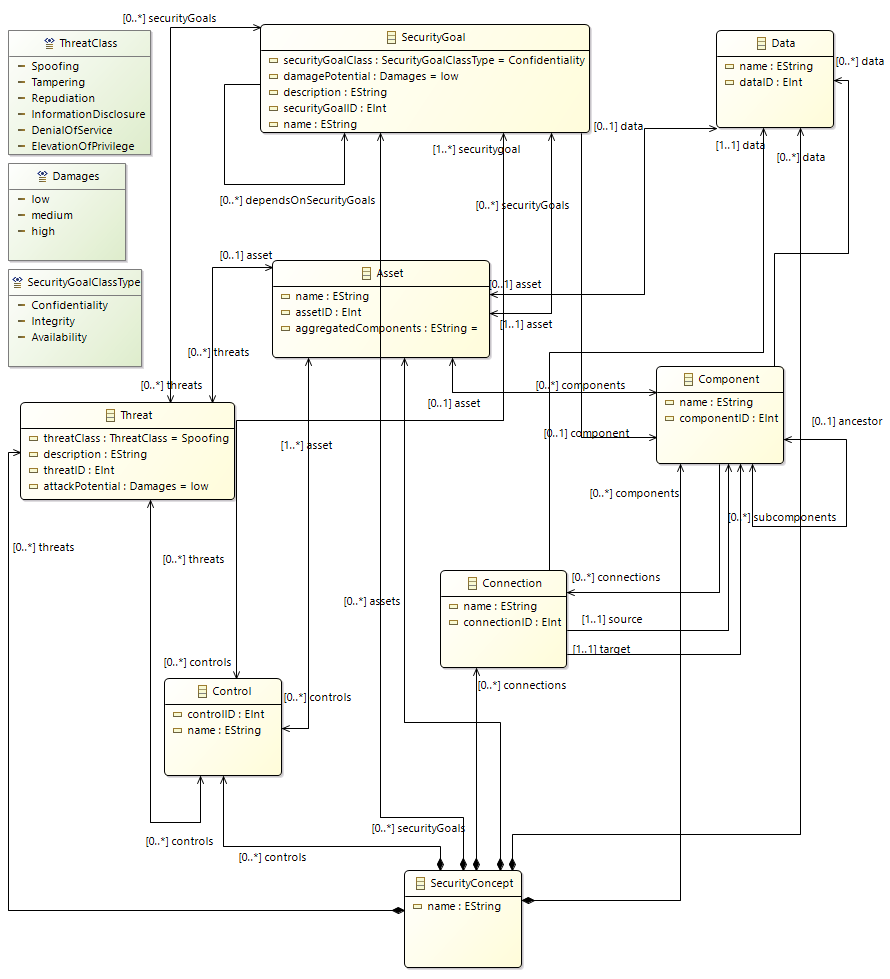
\includegraphics[width=1.2\textwidth]{pictures/concept_metamodel.png}
\caption{Security Concept Metamodel}
\label{fig:concept_metamodel}
\end{figure}

In the figure above all the core elements \textit{Security Goal}, \textit{Asset}, \textit{Control} and \textit{Threat} are pictured. All of these elements are part of a \textit{SecurityConcept}, which in this model will be simply identified by a name. 

SGs have a \textit{Security Goal Class} attribute which describes the purpose of each SG. The \textit{Damage Potential} attribute indicates at the importance of a Goal, i.e. how important it is to secure a certain asset. The higher the damage potential the higher the impact if the security of an asset is breached. One key aspect of this metamodel is the dependency between SGs. A SG is dependent on another SG if both belong to the same asset and have the same security goal class. These dependencies, amongst others, have to be considered during potential transformation steps (Section \ref{subsec:secgoal}). 

Each SG belongs to exactly one asset whereas an asset itself can have unlimited SGs. In this thesis both physical and virtual components can be considered an asset. Both \textit{Data} and \textit{Component} can be assets according to the metamodel. 

There will be two different types of data. For once \textit{processed data}, i.e. data that is being processed or kept in storage by a specific component. On top of that \textit{transmitted data} will be considered separately since the transmission channel itself can be seen as an asset. The resulting interconnections are shown in the following figure:

\begin{figure}[H]
\centering
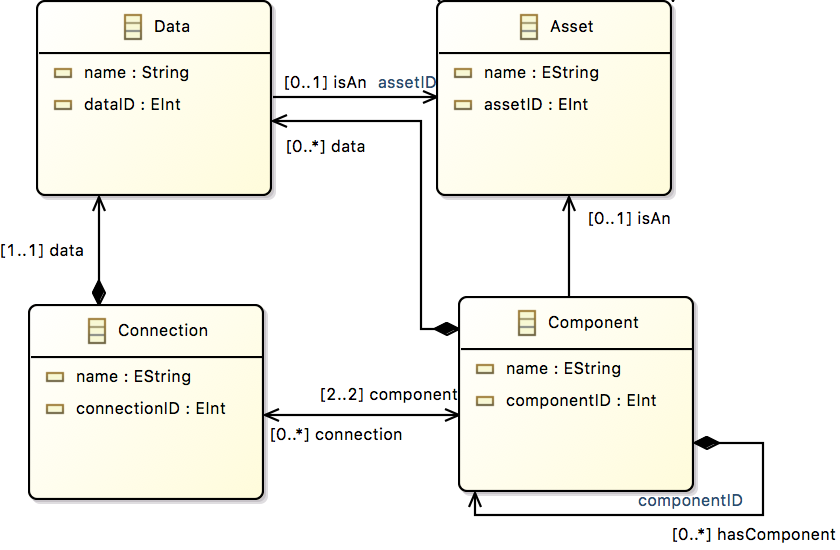
\includegraphics[width=0.65\textwidth]{pictures/two_data.png}
\caption{Two different interpretations of data}
\label{fig:data}
\end{figure} 

As already mentioned data can be viewed as being processed and transmitted. Therefore an element \textit{Connection} was added. A connection is the transmission channel between two components. It must have an associated data. The processed or stored data however can be directly associated with a component. In both cases data can be viewed as an asset. There is no possibility to assign a connection as an asset, the reason being that the transmission medium itself, i.e. the cable, wire, is rarely an object of interest but more so the data which is being transmitted.

Lastly the selection of \textit{Granularity Levels} by users should be enabled. Instead of having two different input models, one security concept model and one model depicting the system structure, one can reproduce the structural properties by adding a reference to the component element.      

\begin{figure}[H]
\centering
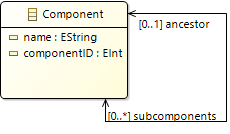
\includegraphics[width=0.45\textwidth]{pictures/component_structure.png}
\caption{Structural information}
\label{fig:data}
\end{figure} 

Having this extra reference one can create infinitely deep structural dependencies within the model. Therefore the actual transformation will only require one model instead of two separate ones.

\subsection{Metamodel elements and their security properties}
To put the different elements of the metamodel into a security context one has to clearly define the Security Goal Classes for possible assets. Interpretations of the classes are not unambiguous and it is necessary to discuss how security attributes propagate through different abstraction layers and what kind of impact interrelated components on different layers have on each other. 

\subsubsection{Components}

Before introducing the transformation rules one has to look at the different kinds of components that can be potentially found in a model instance. Even though the model element remains the same (\textit{Component}) a distinction which is made here is necessary because the interpretation of Security Goal Classes differs depending on the component type. 

\subsubsection*{Physical Component}

Physical components are components that can be accessed physically, e.g. computers, servers, switches etc. Since those can be accessed physically and therefore be manipulated physically one has to define the Security Goal Classes accordingly.

\begin{enumerate}
\item \textbf{Confidentiality} - Will be \textit{undefined} for physical components and will only hold for data stored/processed on those components
\item \textbf{Integrity} - Ensured when the component has not been altered by an adversary in any way; can be broken by an adversary having physical access
\item \textbf{Availability} - Ensured when the component is able to carry out its designated task; can be broken by an adversary having physical access
\end{enumerate}

\subsubsection*{Virtual Component}

Virtual components cannot be directly accessed physically. Examples would be virtual machines, virtual switches etc. The classes are similar to the physical counterpart except from the breach of the respective class.

\begin{enumerate}
\item \textbf{Confidentiality} - Will be \textit{undefined} for virtual components and will only hold for data stored/processed on those components
\item \textbf{Integrity} - Ensured when the component has not been altered by an adversary in any way; can be broken remotely by an adversary, i.e. without having physical access
\item \textbf{Availability} - Ensured when the component is able to carry out its designated task; can be broken remotely by an adversary, i.e. without having physical access
\end{enumerate}

\subsubsection{Data}

Similar to the component element the data element can be interpreted in different ways.
The distinctions between the different data types are very minor but noteworthy nonetheless. We consider three types of data, data which is being stored by a component, data which is being processed by a component and data which is being transmitted between components. The common terminology is \textit{Data at Rest}, \textit{Data in Motion} and \textit{Data in Use} \cite{kanagasingham2008data}. The used terms might be new, the distinction between different states of data however can be found in publications going as far back as 1982, e.g. by Dorothy E. Denning \cite{robling1982cryptography}.

\subsubsection*{Data at Rest}

Data at Rest applies to devices that hold data \cite{kanagasingham2008data}. An example would be a database containing sensitive information. The database being the \textit{Virtual Component} and the stored data being the \textit{Data at Rest}. One could also define the server with the database as a \textit{Physical Component}.

\begin{enumerate}
\item \textbf{Confidentiality} - Ensured when the data is protected from unauthorized disclosure at rest
\item \textbf{Integrity} - Ensured when the data is protected from unauthorized modification at rest
\item \textbf{Availability} - Ensured when the data is available to authorized parties when needed, i.e. authorized parties can access and use the data when needed
\end{enumerate}

\subsubsection*{Data in Use}

Data in Use applies to data that is being processed by a component, i.e. is being used by a service running on a component. An example would be data that is being processed by an API on a server. The API being the \textit{Virtual Component} and the server being the \textit{Physical Component}. The \textit{Data in Use} would be the processed information by the API backend.

\begin{enumerate}
\item \textbf{Confidentiality} - Ensured when the data is protected from unauthorized disclosure during processing
\item \textbf{Integrity} - Ensured when the data is protected from unauthorized modification during processing
\item \textbf{Availability} - Ensured when the data is available to authorized parties when needed, i.e. the data is being processed by the service/the respective service is running when needed
\end{enumerate}

\subsubsection*{Data in Motion}

Data in Motion applies to all data transmitted between components. We do not specify any protocols here to keep the definition as broad as possible.

\begin{enumerate}
\item \textbf{Confidentiality} - Ensured when the data is protected from unauthorized disclosure during transmission
\item \textbf{Integrity} - Ensured when the data is protected from unauthorized modification during transmission
\item \textbf{Availability} - Ensured when the data is available to authorized parties when needed, i.e. is not lost or intercepted during transmission 
\end{enumerate}

The different component/data types shown here should only show the different interpretations of the elements of the security concept metamodel. The interpretation of the element itself does not have an influence on the chosen metamodel element, i.e. the element for both physical and virtual components will still be \textit{Component}. The only difference can be found in data since transmitted data always belongs to a \textit{Connection}. For both processed and stored data however the metamodel element \textit{Data} will be used.

\subsubsection{Interpretation of Interconnections between Elements}

To describe model transformations in the security context one has to discuss how exactly the security attributes propagate through the respective abstraction layers. Here we will look into the dependencies between components and their security properties during transformations.

\subsubsection*{Sub-component}
\label{subsubsec:sub_comp}
A sub-component \textit{SC} will be defined as a component that directly belongs to a component \textit{C} which is in an abstraction layer above, i.e. encapsulates one or more sub-components. According to the previously defined metamodel such a relationship between components is being defined by the \textit{hasComponent} composition, i.e. a sub-component cannot exist without a component here. This also means that no new data types or structures are added when changing to higher granularity levels. Sub-components can only process data that has already been defined in the layers above. An example would be a database encapsulating a sub-component such as a secure key storage.   

\subsubsection*{Security Goals}
\label{subsubsec:sec_goal}
For security goals the interconnections between components and sub-components have to be interpreted in an unambiguous way. There is no clear definition on how SGs for components in higher abstraction layers propagate to the respective sub-components in the abstraction layers below. We therefore adopt the idea for security requirements which was proposed by Menzel et al. \cite{Menzel2008}. Here, the main focus will be on two characteristics, \textit{Independent} and \textit{Require} to capture interdependencies between SGs on different granularity levels. According to the metamodel each SG has the following attributes:

\begin{figure}[H]
\centering
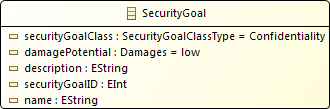
\includegraphics[width=0.65\textwidth]{pictures/securitygoal.png}
\caption{Attributes of a Security Goal}
\label{fig:security_goal}
\end{figure} 

The key attributes are \textit{securityGoalClass} and \textit{damagePotential}. Both are relevant when it comes to aggregation rules and dependencies amongst components. In this chapter the focus will be on the latter.

In case of a complete security concept definition interdependencies amongst components and security goals are clear, similar to Figure \ref{fig:subcomponent}. Out of simplicity security goals will be linked directly to components and not through assets.

\begin{figure}[H]
\centering
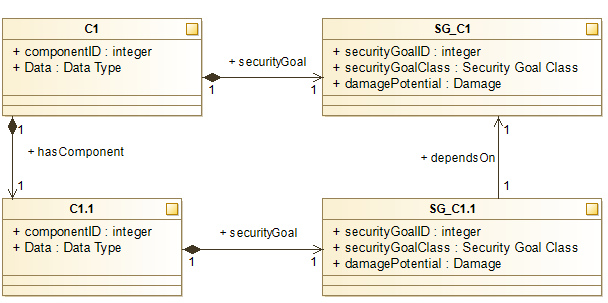
\includegraphics[scale=0.75]{pictures/rel_component.png}
\caption{Relationships between Security Goals}
\label{fig:subcomponent}
\end{figure} 

Figure \ref{fig:subcomponent} has shown the dependencies between components and their security attributes in case of a complete security concept definiton. In underspecified security concepts, such as shown in Figure \ref{fig:subcomponent_dilemma}, the dependencies are not as trivial. 

\begin{figure}[H]
\centering
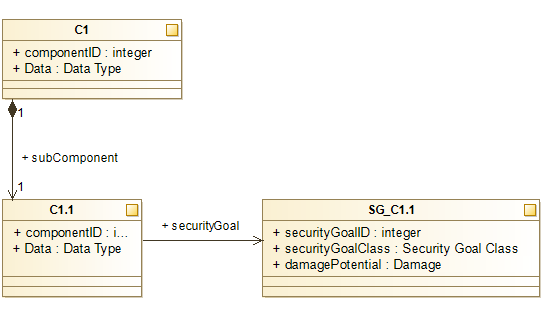
\includegraphics[width=0.75\textwidth]{pictures/sg_dilemma_no_goal.png}
\caption{Ambiguous propagation}
\label{fig:subcomponent_dilemma}
\end{figure} 

It is not obvious what kind of influence the sub-component has on its parental node, if at all. If the confidentiality of component $C_{1.1}$ is protected it is not clear how it will propagate to higher abstraction layers. Similar observations can be made for the aggregation from higher abstraction layers to lower ones. One has therefore to define when and how security attributes will propagate based on structural features of the SUS.

\begin{theorem}
A security goal $SG_{C_1}$ of a component $C_1$ has a direct influence on another component $C_2$ if and only if there is: 
\begin{enumerate}
\item a direct link between the two components, i.e. a hierarchical relationship between the two components AND
\item component $C_2$ processes/holds the data type that is being addressed by $SG_{C_1}$
\end{enumerate} 
\end{theorem}

This \textit{direct influence} is one of the more obvious dependencies amongst components. At first glance matching data types are needed to aggregate SGs through different abstraction layers but it is certainly possible that security concepts might be underspecified. Relying on this definition might therefore severely limit the transformation and thus, the resulting model.

An exemplary model instance follows showing security attribute propagation with an underspecified security concept. Similarly to previous examples data/components will be directly linked with security goals without asset elements in between in the interest of greater clarity.

\begin{figure}[H]
\centering
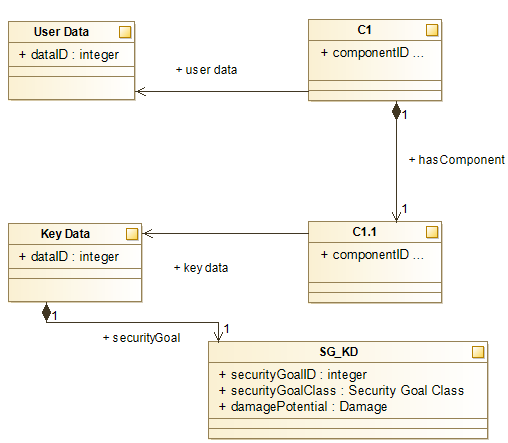
\includegraphics[width=0.75\textwidth]{pictures/sg_deduction.png}
\caption{Ambiguous propagation}
\label{fig:subcomponent_dilemma}
\end{figure} 

The corresponding security goal of the key data in natural text could be:

\begin{itemize}
\item[]\textbf{$SG_{KD}:$} The Confidentiality of sensible key data should be protected
\end{itemize}

Now we will look at component $C_{1.1}$ which has a link to key data. When looking through its SGs we will only find $SG_{KD}$ which should protect the \textit{Confidentiality} of said data. There is also a direct connection from $C_{1.1}$ to component $C_1$ which is in a granularity level above. 

According to the definition (Section \ref{subsubsec:sub_comp}) a sub-component can only process data that already exists in the abstraction layers above. Thus, a correct conclusion would be that if the confidentiality of key data is protected in $C_{1.1}$ it is also protected in the layer above even though there is no explicit link between $C_1$ and key data. This however, does \textit{NOT} mean that the overall confidentiality is being protected since $C_1$ may process other data, such 
as user data in the example.

Propagation from higher layers to lower ones is generally not possible without explicit links to data types. This will be discussed more thoroughly in Section \ref{subsec:sec_goals_rules}.

Similar conclusions can be made for the \textit{Integrity} of sub-components and its propagation to abstraction layers with higher or lower granularity levels with one slight difference. When looking at components at higher abstraction layers we can say that if the integrity of a component $C_1$ is being protected then all of its sub-components are being protected as well. 

For \textit{Availability} however, the situation differs. The connection between components (\textit{hasComponent}) has been defined as a composition. This means that the availability of a specific sub-component is pre-determined by the structural features of the SUS. If the availability of a component $C_1$ is protected it necessarily means that the availability of its sub-components is protected as well. To have the availability of a component protected however all of the sub-components have to be protected individually. The availability of a component is therefore the union of availabilities of its sub-components.

\subsubsection*{Threats}

Similar to SGs one can look into propagation rules for threats. Firstly we will look at the important attributes of a threat. The key attribute here will be \textit{attackPotential} which will be considered during the transformation steps in Section \ref{subsec:sec_goals_rules}.  
 
\begin{figure}[H]
\centering
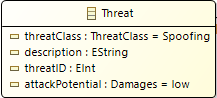
\includegraphics[scale=0.85]{pictures/threat.png}
\caption{Attributes of a Threat}
\label{fig:threat}
\end{figure} 

Here, the focus will be on the propagation of threats through granularity levels based on an underspecified security concept.

Every defined threat threatens at least one SG according to the metamodel (Figure \ref{fig:concept_metamodel}) and since every SG addresses one asset (component or data) we can adapt the observations made in the previous section. 

\begin{figure}[H]
\centering
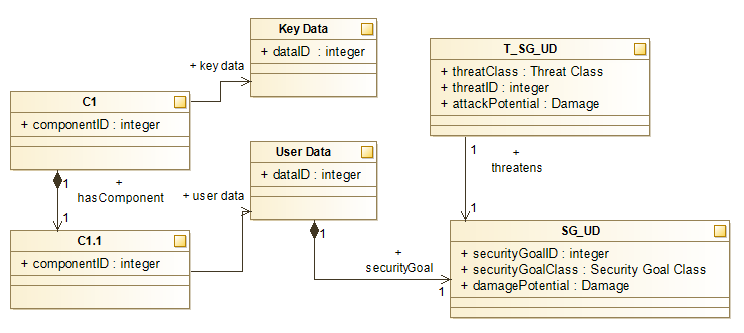
\includegraphics[scale=0.85]{pictures/threat_overview.png}
\caption{Underspecified Security Concept with a Threat}
\label{fig:threat_overview}
\end{figure} 

In Figure \ref{fig:threat_overview} a threat $T_{SG_{UD}}$ threatens $SG_{UD}$ which addresses the user data that is being used by sub-component $C_{1.1}$. The influence of $T_{KD}$ on higher abstraction layers is of interest since neither SGs nor threats are explicitly defined in the example.

\begin{itemize}
\item[]\textbf{$SG_{UD}:$} The Confidentiality of sensible user data should be protected
\item[]\textbf{$T_{SG_{UD}}:$} Eavesdropping on sensible user data
\end{itemize}

Similar to SGs, we can assume that $T_{SG_{UD}}$ propagates to the layer above based on the definition of sub-components. User data, which is only explicitly addressed by $SG_{UD}$, is also present at parental nodes. Thus, if the \textit{Confidentiality} of user data is being threatened by $T_{SG_{UD}}$, it is also being threatened when looking at $C1$.

For the propagation from abstraction layers depicting lower granularities ($C_1$) to layers with higher granularity ($C_{1.1}$) we have to take the data types into account. We will define a SG addressing key data and the corresponding threat.

\begin{itemize}
\item[]\textbf{$SG_{KD}:$} The Confidentiality of key data should be protected
\item[]\textbf{$T_{SG_{KD}}:$} Disclosure of key data
\end{itemize}

Now if the the confidentiality is being threatened by $T_{SG_{KD}}$ it is not clear how it will propagate to the layers below since $C_{1.1}$ is not addressing key data in any observable way. 

Threats that threaten SGs with \textit{Integrity} as their security goal classes behave differently. Contrary to confidentiality, assumptions can be made when looking at propagation from higher abstraction layers to lower ones. When integrity of a component $C_n$ is being threatened the integrity of all respective sub-components $C_{n.1} ... C_{n.m}$ is being threatened as well. If the integritiy of a sub-component $C_{n.i}$ is being threatened it will also propagate to its parental node $C_n$ since a node can only be as secure as its sub-nodes.

Lastly, for \textit{Availability} the propagation is pre-determined by the structural features and the definition of sub-components. If the availability of a component $C_n$ is threatened it propagates to its sub-components $C_{n.1} ... C_{n.m}$. 

If the availability of one sub-component is being threatened it will also propagate to its parental nodes. This however does not provide information on how severely the availability of $C_n$ as a whole will be impaired in case of an attack on the availability of $C_{n.i}$. This propagation from sub-components to their parental nodes is very similar to the just mentioned integrity behavior. The availability of $C_n$ is a union of availabilities of its sub-components and one threat on a specific $C_{n.i}$ would alter said set.

We can therefore conclude that to ensure a SG of a component $C_n$ all its sub-components have to be protected as well. For threats however it is enough to threaten one sub-component to have an effect on its parental node.

\subsubsection*{Controls}

Controls try to mitigate threats and are directly linked to at least one threat at all times. The propagation of controls through abstraction layers will therefore be closely coupled with threats and SGs.

\begin{figure}[H]
\centering
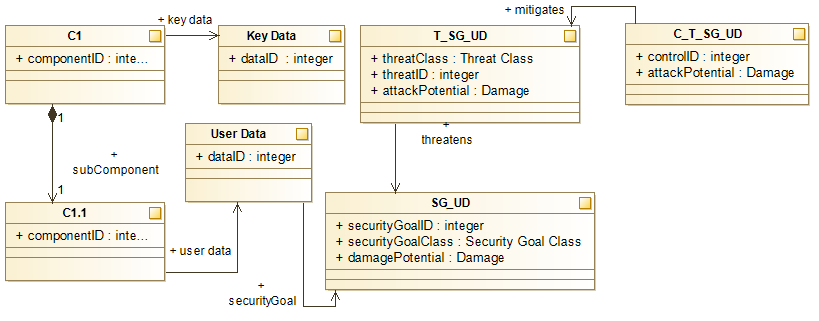
\includegraphics[width=\textwidth]{pictures/control_propagation.png}
\caption{Underspecified Security Concept with a Control}
\label{fig:control_propagation}
\end{figure} 

We have already discussed the propagation of SGs and threats in the previous chapters and thus, indirectly the propagation of controls. The example in Figure \ref{fig:control_propagation} shows a control that mitigates the threat $T_{SG_{UD}}$. In natural text the security attributes could be the following:

\begin{itemize}
\item[]\textbf{$SG_{KD}:$} The Confidentiality of sensible user data should be protected
\item[]\textbf{$T_{SG_{KD}}:$} Eavesdropping on sensible user data
\item[]\textbf{$C_{T_{SG_{KD}}}:$} Encryption of sensible user data with AES-256 to pevent eavesdropping
\end{itemize}

Similar to threats which propagate to the upper abstraction layers, controls will as well. The rules will be the same since the controls are very tightly coupled and cannot exist without threats.

For this example this would mean that when looking at the abstraction layer above and at $C_1$ we will consider the control $C_{T_{SG_{KD}}}$ as well the threat $T_{SG_{KD}}$ it is mitigating.

This section was only giving an overview on the conclusions for security attributes that can be made based on the structural features of an (underspecified) security concept definition. A more thorough definition will be discussed in the following section. 

\subsection{Model Transformation}

Let $SG_{CIA}(SUS)$ be the set of security goals for a SUS. A security goal SG is defined as $SG(cl, c, asset, dmg)$ where $cl$ is the security goal class ($C$ for confidentiality, $I$ for Integrity and $A$ for availability), $c$ being the component, $asset$ being the element of interest which the SG was defined for, i.e. the component itself or data which is being processed by it and $dmg$ is the damage potential in case of a security breach ($H$ = high, $M$ = medium and $L$ = low).

Similarly we define a threat set $T_{STRIDE}$ for a SUS where STRIDE is the threat modeling technique developed by Microsoft. According to \cite{torr} a component can be exposed to the following threats:

\begin{enumerate}
\item[]\textbf{Spoofing:} Adversaries pretend to be someone else
\item[]\textbf{Tampering:} Adversaries change data in transit
\item[]\textbf{Repudiation:} Adversdaries perform actions that can't be traced back to them
\item[]\textbf{Information disclosure:} Unauthorized viewing/stealing of data
\item[]\textbf{Denial of service:} Interruption of system services
\item[]\textbf{Elevation of privilege:} Performing of unauthorized actions
\end{enumerate}

Every threat has therefore a specific threat class that it can be assigned to. $T_{STRIDE}$ is the set of threats where $T(tc, sg, sev)$ is a threat, $tc$ being the threat class, $sg$ being the security goal which the threat violates and $sev$ being the severity of the threat if successfully exploited ($H$ = high, $M$ = medium and $L$ = low). 

Controls are tightly coupled with security goals and threats. $C_{SUS}$ is the set of controls for a SUS that contains all the controls. A Control $C(T)$ has a set of threats $T$ it mitigates.

Each asset can be viewed separately when looking at security goals and threats. For SGs we can define three separate sets, $SG_C(c)$, $SG_I(c)$ and $SG_A(c)$ where each one contains the respective SGs with either confidentiality, integrity or availability as the security goal class.

\begin{theorem}
$SG_{CIA}(c) = SG_C(c) \cup SG_I(c) \cup SG_A(c)$
\end{theorem}

The respective sets covering one security goal class can be defined as follows:

\begin{theorem}
$SG_{sgc}(c) = SG(sgc, c, asset_j, dmg) \cup SG(sgc, c, asset_{j+1}, dmg)  \cup ... \cup SG(sgc, c, asset_m, dmg) $
\end{theorem}

%
%Furthermore we define that for every component $C$ the SG sets are the union of the SGs of its sub-components with the same security goal class. For the confidentiality we have to consider pairs of components and data, since confidentiality is only defined on data. Therefore when looking at a component $c_i$ and a data asset $asset_{d_{j}}$ we can say that the confidentiality of data $d_j$ for component $c_i$ is the union of the SGs of its sub-components also covering $d_j$. $sgc$ is either confidentiality ($C$), integrity ($I$) or availability ($A$).
% 
%\begin{theorem} 
%$SG_{sgc}(c_i, asset_{d_{j}}) = SG_{sgc}(c_{i_{1}}, asset_{d_{j}}) \cup ... \cup SG_{sgc} (c_{i_{n}}, asset_{d_{j}}) $
%\end{theorem}
%
%The unions for data assets for integrity and availability can be created accordingly.
%
%For non-data assets the union set is very similar with the security goal class being either integrity or availability.
%
%\begin{theorem} 
%$SG_{sgc}(c_i, asset_{c_{i}}) = SG_{sgc}(c_{i_{1}}, asset_{c_{i_{1}}}) \cup ... \cup SG_{sgc} (c_{i_{n}}, asset_{c_{i_{n}}}) $
%\end{theorem}

Threats can be defined accordingly. For a threat $T$ with the threat class $tc$ the following union set can be defined. 

\begin{theorem} 
$T_{tc}(c) = T(tc, sg_i, sev) \cup T(tc, sg_{i+1}, sev) \cup ... \cup T(tc, sg_n, sev) | sg_i \in SG_{CIA}(c)$
\end{theorem}

The set $T_{STRIDE}$ ist therefore a union of all threat sets:

\begin{theorem} 
$T_{STRIDE}(c) = T_S(c) \cup T_T(c) \cup T_R(c) \cup T_I(c) \cup T_D(c) \cup T_E(c)$
\end{theorem}

The just mentioned sets are the basic sets for components without looking at structural features of a SUS. As mentioned in Section \ref{subsec:interpretation} we can derive further security properties from sub-components and overall structural features of the system. This derivation will be covered in the following Sections.

\subsection{Transformation Rule Set for Security Goals}
\label{subsec:sec_goals_rules}

The transformation rules for security goals will now be introduced. The following pseudocode will then be explained afterwards using an exemplary security concept. The function  \texttt{compute\_SG} has two inputs, $cid$ is  an ID of the component selected by the user and \texttt{security\_concept} is the initial security concept model. The user-selected component IDs display the granularity level. The user can select as many components as needed and the result will be a security concept with the aggregated security attributes for the selected elements.

\begin{algorithm}[H]
\caption{Transformation rules for security goals}
security\_concept $\gets$ \text{security concept model} \\
$L_v$ $\gets$ \text{list of visited nodes} \\
$L_c$ $\gets$ \text{list of components of interest} \\
$L_{sg}$ $\gets$ \text{list of security goals} \\
$S_{anc}$ $\gets$ \text{ancestor node stack} \\
$S_{subc}$ $\gets$ \text{children node stack} \\

\begin{algorithmic}[1]

\Function{compute\_sg}{$cid$, security\_concept}
\State $L_{sg}$ $\gets$ empty
\State $component$ = findComponentByID($cid$)
\If {$component$ not in $L_v$}
\State $L_v$.add($component$) \label{line:visited}
\ForAll{sg in $component$.asset.securityGoals} \label{line:iterate_own_sg}
	\State $L_{sg}$.add(sg)	
\EndFor
\ForAll{con in $component$.connections}
\State $L_{sg}$.add(con.data.asset.securityGoal)
\EndFor
\State findAncestors($component$) 
\State findChildren($component$) 
\State checkConnections($L_{sg}$, $component$)
\State securityGoalAggregation({$L_{sg}$})
\State writeToSecurityConcept($cid$, $L_{sg}$) 
\Else
\State break
\EndIf
\EndFunction

\Function{findAncestors}{$component$, $child$}
\If{$component$.Ancestor} 
\If{$component$.Ancestor in $L_c$}
\State{$S_{anc}$.add($component$.Ancestor)} 
\State{findAncestors($component$.Ancestor, $child$)}
\EndIf
\State add\_sg\_anc($component$.Ancestor, $component$)
\State findAncestor($component$.Ancestor, $child$)
\Else
\ForAll{cmp in $S_{anc}$}
\State sg\_compute($cmp.id$, security\_concept) \label{line:ancestor}
\State add\_sg\_anc($cmp.id$, $component$)
\EndFor
\EndIf

\EndFunction
\algstore{testcont} 

\end{algorithmic}
\end{algorithm}

\begin{algorithm}[H] 
\begin{algorithmic}
\algrestore{testcont} 

\Function{findChildren}{$component$, $anc$}
\If{$component$.SubComponents}
\ForAll{cmp in $component$.SubComponents} \label{line:subcomponent}
\If{cmp in $L_c$}
\State{$S_{subc}$.add($cmp$)} 
\State{findChildren($cmp$, $anc$)}
\State{fixConnection($component$, $cmp$)} \label{line:connection}
\EndIf
\State add\_sg\_child($cmp$, $component$)
\State fixConnection($component$, $cmp$)
\State findChildren($cmp$, $anc$)
\EndFor
\Else
\ForAll{cmp in $S_{subc}$}
\State sg\_compute($cmp.id$, security\_concept)
\State add\_sg\_child($cmp$, $component$)
\EndFor
\EndIf
\EndFunction

\Function{add\_sg\_AtoC}{$anc$, $child$} \label{line:anc_child} \Comment{ancestor to child} 
\ForAll {asset in $anc$.assets}
\ForAll {sg in $anc$.asset.securityGoals}
\If($asset.componentID$ == $anc$.id)
\State sg.c = $child$
\State sg.asset = $child$
\State $child$.asset.securityGoals.add(sg)
\ElsIf{sg.securityGoalClass == 'Confidentiality' \&\& sg.asset in $child$.assets}
\State sg.c = $child$
\State $child$.asset.securityGoals.add(sg)
\ElsIf{sg.securityGoalClass == 'Integrity' || 'Availability'}
\State sg.c = $child$
\State $child$.asset.securityGoal.add(sg)
\EndIf
\EndFor
\EndFor
\EndFunction

\algstore{testcont}
\end{algorithmic}
\end{algorithm}

\begin{algorithm}[H] 
\begin{algorithmic}
\algrestore{testcont} 

\Function{add\_sg\_CtoA}{$child$, $anc$} \label{line:child_anc} \Comment{child to ancestor}
\ForAll {asset in $child$.assets}
\ForAll {sg in $child$.asset.securityGoals}
\If{!$anc$.assets.contain($child$.asset)}
\State copyAsset($child$.asset, $anc$) \label{line:asset_copy}
\ElsIf{sg.securityGoalClass == 'Confidentiality'}
\State sg.c = $anc$
\State $anc$.asset.securityGoals.add(sg)
\ElsIf{sg.securityGoalClass == 'Availability'}
\State sg.c = $anc$
\State $anc$.asset.securityGoal.add(sg)
\EndIf
\EndFor
\EndFor
\EndFunction

\Function{fixConnection}{$child$, $anc$}
\ForAll {con in $child$.connections}
\If {con.source == $child$}
\State con.source = $anc$
\ElsIf {con.target == $child$}
\State con.target = $anc$
\EndIf
\EndFor
\EndFunction

\Function{checkConnections}{$L_{sg}$, $component$}
\ForAll {con in $component$.connections}
\If {(con.source || con.target) not in $L_c$}
\State $component$.connections.delete(con)
\Else
\State $L_{sg}$.addEach(con.data.asset.securityGoals)
\EndIf
\EndFor
\EndFunction

\algstore{testcont}
\end{algorithmic}
\end{algorithm}

\begin{algorithm}[H] 
\begin{algorithmic}
\algrestore{testcont} 

\Function{securityGoalAggregation}{$L_{sg}$}
\State final\_sgs $\gets$ empty
\ForAll {sg in $L_{sg}$}
\State tmp\_sg = $L_{sg}$.where(\_sg.securityGoalClass == sg.securityGoalClass  \&\& \_sg.asset == sg.asset)
\State tmp\_sg.first.damagePotential = tmp\_sg.where(damagePotential.max)
\State final\_sgs.add(tmp\_sg.first)
\EndFor
\EndFunction
\end{algorithmic}
\end{algorithm}

\subsubsection{Model Transformation using an Example}

The following security concept serves as an example. The selected granularity level is displayed by the three marked components, $C1$, $C2$ and $C1.1.1$. Some of the components in the security concept have security goals defined. The goal now is to derive the influence these goals have on the selected components. In this chapter a complete transformation will be carried out and the resulting security concept will be presented. Key transformation steps will be discussed and highlighted.

\begin{figure}[H]
        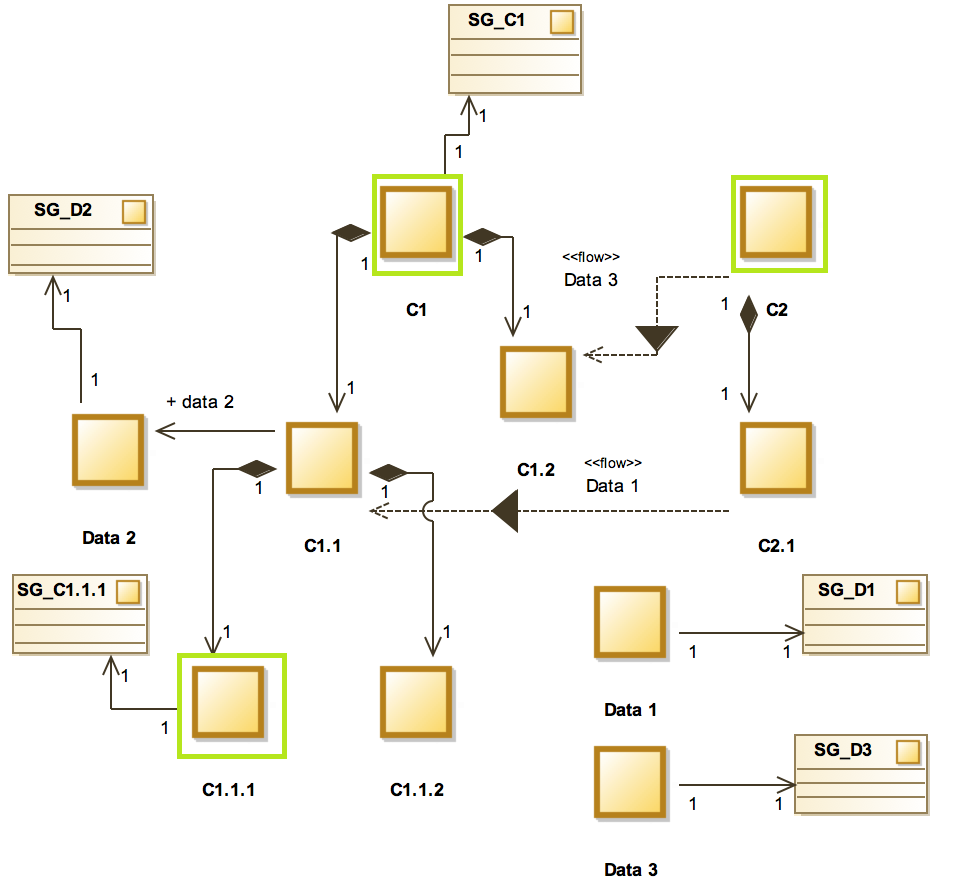
\includegraphics[width=1\linewidth]{pictures/sg_transformation}
    \caption{Security Concept Model}
\end{figure}

For every component of interest the function $compute\_sg$ will be called. First the list of components $L_c$ will be populated with the three component s $C1$, $C2$ and $C1.1.1$. Prior to applying the algorithm, we have to define the security goals. A definition follows:

\begin{align*}
SG_{CIA}(sec\_concept) = \{SG(A,C1.1.1,C1.1.1,"high") &, \\ SG(C,C1.1,D2,"medium")&, \\
SG(I,C1,C1,"low")&, \\
SG(C,-,D1,"high")&, \\
SG(C,-,D3,"medium")\} 
\end{align*}

To cover as many cases as possible we will start with component $C1.1.1$. The first step, as seen in line \ref{line:iterate_own_sg}, is to add all the security goals of the component to its security goal list $L_{sg}$. We only have one goal to address and therefore the set will only have one element.

\begin{align*}
L_{sg} = \{SG(A,C1.1.1,C1.1.1,"high")\}
\end{align*}

Now, we will have to look at the ancestors/children of the node. We differentiate between two kinds of ancestors, an ancestor that is in $L_c$ and is therefore a component of interest and an ancestor that is not in $L_c$. Ancestors that are in $L_c$ have to processed individually (line \ref{line:ancestor}).

$C1.1$ is not in $L_c$ and therefore only the function $add\_sg\_AtoC$ will be called (line \ref{line:anc_child}). $SG\_D2$ is the only security goal for component $C1.1$ but since Data 2 is not an asset of the sub-component $C1.1.1$, it will not propagate to the abstraction layer below. $findAncestor$ is then called with the ancestor of $C1.1$, i.e. $C1$.

Since $C1$ is in $L_c$ it will be added to the ancestor stack that the algorithm will have to work through. This is important in cases where there is a chain of components that are all in $L_c$. In such case, we would have to iterate through all of those nodes starting with the one in the highest abstraction layer. $C1$ does not have an ancestor and therefore the function $sg\_compute$ for $C1$ will be called (line \ref{line:ancestor}).

Every time $sg\_compute$ is being called the respective component is being added to the list of visited nodes ($L_v$) to ensure that nodes would not be processed multiple times (line \ref{line:visited}). After calling $sg\_compute$ with $C1$ as the component, our list is now:

\begin{align*}
L_v = \{C1.1.1, C1\}
\end{align*}

Analogous to $C1.1.1$, the security goals of $C1$ will be added to $L_{sg}$.

\begin{align*}
L_{sg} = \{SG(I,C1,C1,"low")\}
\end{align*}

Since $C1$ does not have any ancestor nodes, the function $findChildren$ will be called.  Every sub-component of the current component will be processed (line \ref{line:subcomponent}). Similar to the ancestor function we differentiate between two kinds of children, ones that are in $L_c$ and ones that are not.

$C1$ has two sub-components $C1.1$ and $C1.2$ that have to be processed as well. We start with $C1.1$ which is not in $L_c$ and therefore $C1.1$ will not be added to the sub-component stack $S_{subc}$. The security goals however will be added to $L_{sg}$ which still belongs to the ancestor $C.1$. The component must be altered. The initial security goal had $C1.1$ as the component which must be changed to $C1$. Moreover must one ensure that the asset exists in the layer above. This is not the case for $C1$ and therefore Data 2 will be copied and inserted into the abstraction layer above (line \ref{line:asset_copy}).

\begin{align*}
L_{sg} = \{SG(I,C1,C1,"low"), SG(C,C1,D2, "medium")\}
\end{align*}

After having the security goal added we will proceed with the sub-component of $C1.1$, namely $C1.1.1$. The function $find\_children$ is being called recursively with two parameters, the current component $component$ which is $C1.1$ here and the initial parental node $anc$. This way the security attributes will be correctly aggregated regarding $anc$.

$C1.1.1$ has one security goal, $SG\_C1.1.1$ that addresses the availability of the component. Since there are no further children $add\_sg\_CtoA$ will be called. According to the idea presented in Section \ref{subsubsec:sec_goal} the protection of the availability of a sub-component does not necessarily mean the availability of the components in higher abstraction layers. Thus, $SG\_C1.1.1$ will not be added to $L_{sg}$. The other sub-component $C1.1.2$ does not possess any security attributes and does not have any influence on its ancestors.

The function $fixConnection$ that is called while processing the sub-components has not yet been addressed. The nodes $C1.1.1$ and $C1.1.2$ do not have connections to other components, $C1.1$ however, does. After iterating through the sub-components of $C1.1$ this function is being called. 

The connection, that would be otherwise lost during abstraction, has to be processed. The connection that has $C1.1$ as the target will be changed in a way that $C1$ becomes the target. This way potential security attributes that address this connection and the data being transmitted on it will not be lost during the transformation. The following figure depicts the changed connection.

\begin{figure}[H]
\centering
\begin{subfigure}{.5\textwidth}
  \centering
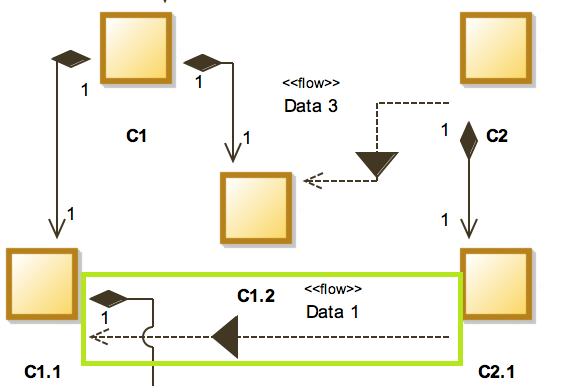
\includegraphics[width=0.73\textwidth]{pictures/initial}
\caption{Before connection adjustment}
\label{fig:con_c1.1}
\end{subfigure}%
\begin{subfigure}{.5\textwidth}
  \centering
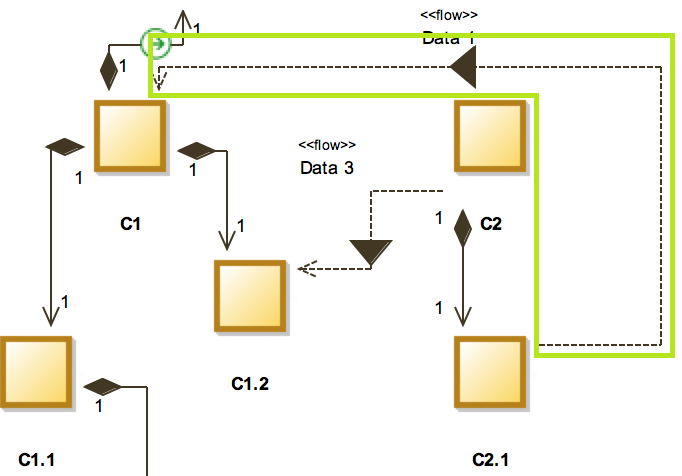
\includegraphics[width=0.7\textwidth]{pictures/con_c11}
\caption{After connection adjustment}
\label{fig:con_c1.1}
\end{subfigure}
\label{fig:test}
\end{figure}

When processing the second sub-component of $C1$ we find another connection that needs to be addressed as well. The target is being changed from $C1.2$ to $C.1$ as the following figure suggests.

\begin{figure}[H]
\centering
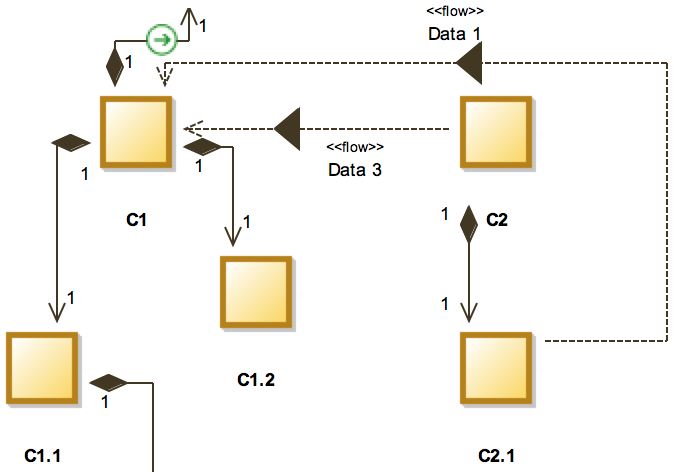
\includegraphics[width=0.7\textwidth]{pictures/con_c12}
\caption{Underspecified Security Concept with a Control}
\label{fig:con_c1.2}
\end{figure} 

Lastly the function $checkConnections$ will be called to verify that both sources and targets of the added connections are in $L_c$. Only then will the security attributes be added to the resulting model. In this case only one connection is correct having both the source and target in $L_c$. Therefore we will add the security goals addressing the transmitted data Data 3. The other connection will be deleted for now since the source is not in $L_c$.

\begin{align*}
SG_{CIA}(C1) = \{SG(I,C1,C1,"low"), SG(C,C1,D2, "medium"), \\ SG(C,-,D3,"medium")\}
\end{align*}

The aggregation for $C1$ has been carried out while iterating through the ancestors of $C1.1.1$. To conclude the aggregation the function $add\_sg\_AtoC$ will be called. $C1$ now has two security goals that might have an influence on $C1.1.1$. In Section \ref{subsubsec:sec_goal} the propagation of security attributes through abstraction layers has been discussed. If the integrity for a component $C$ is being protected it necessarily means that the integrity of its sub-components $C_i ... C_n$ is being protected as well. We can therefore add $SG\_C1$ to $L_{sg}$ for $C1.1.1$ while adjusting the properties of the security goal. The attributes component and assets will be changed from $C1$ to $C1.1.1$.

\begin{align*}
SG_{CIA}(C1.1.1) = \{SG(A,C1.1.1,C1.1.1,"high"), SG(I,C1.1.1,C1.1.1,"low")\}
\end{align*}

There is one final component that has to be addressed. $C2$ is in $L_c$ and similar to the previous nodes the function $compute\_sg$ will be called. $C2$ has no direct security attributes and no ancestors. The only component is the child $C2.1$ that has a connection to $C1$. 

While processing $C2.1$ the function $fixConnection$ will be called that will  put its ancestor as the source of the connection. The resulting model follows.

\begin{figure}[H]
\centering
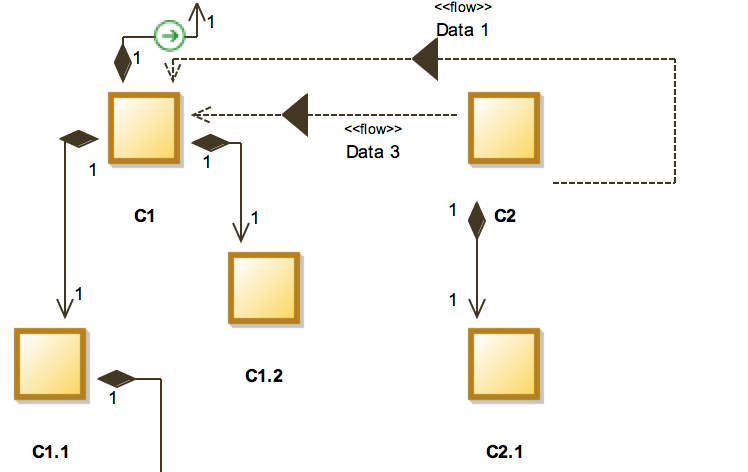
\includegraphics[width=0.7\textwidth]{pictures/con_c2}
\caption{Underspecified Security Concept with a Control}
\label{fig:con_c2}
\end{figure}

$checkConnections$ will be called at last and both outgoing connections will be processed. Since targets and sources are in $L_c$ security attributes of both connections will be added to the security goal set of $C2$. 

\begin{align*}
SG_{CIA}(C2) = \{SG(C,-,D1,"high"), SG(C,-,D3,"medium")\}
\end{align*}

One more iteration is needed to assure that all connections of all components have been added correctly. As a result a security goal addressing Data 1 will be added to the security goal set of $C1$.

\begin{align*}
SG_{CIA}(C1) = \{SG(I,C1,C1,"low"), SG(C,C1,D2, "medium"), \\ SG(C,-,D3,"medium"), SG(C,-,D1,"high")\}
\end{align*} 

The transformation result as well as a comparison between the initial set of security attributes and the resulting set follows.

\begin{figure}[H]
\centering
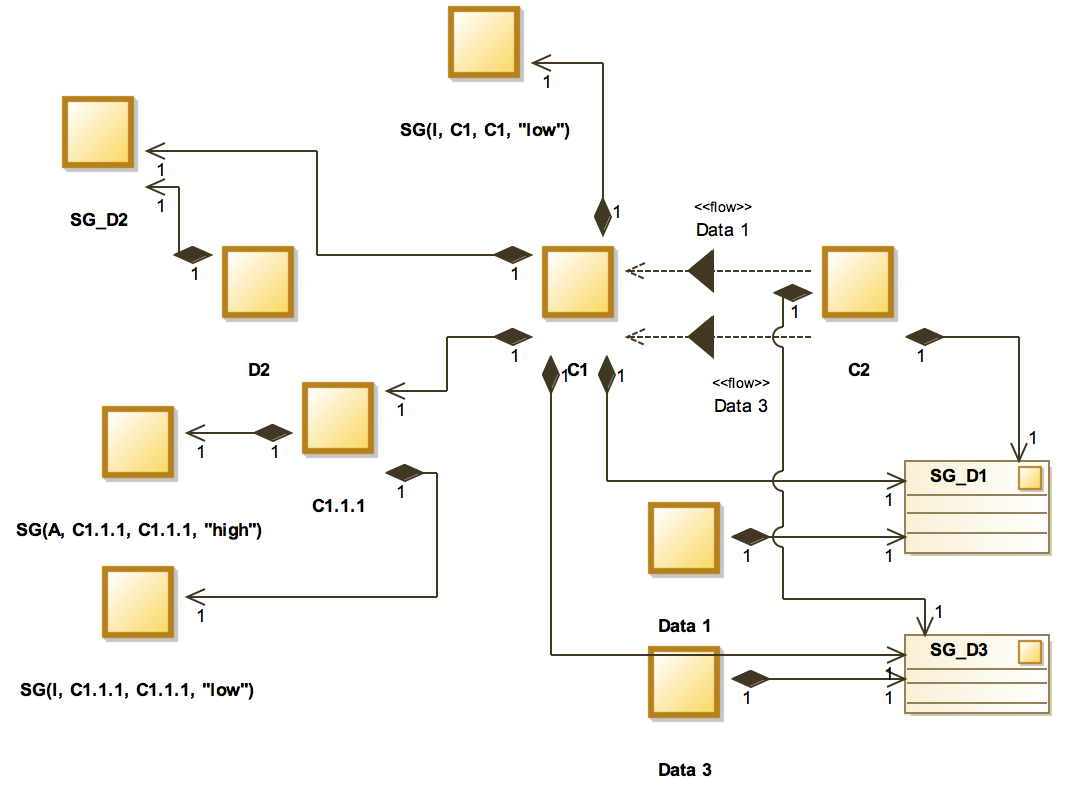
\includegraphics[width=0.7\textwidth]{pictures/finished_transformation}
\caption{Security concept after the transformation}
\end{figure} 


\begin{align*}
SG_{CIA}(C1) = \{SG(I,C1,C1,"low")\}\\
SG_{CIA}(C1.1.1) = \{SG(A,C1.1.1,C1.1.1,"high")\}\\
SG_{CIA}(C2) = \emptyset
\end{align*}

\begingroup\vspace*{-\baselineskip}
\captionof{figure}{Security goal set before aggregation}
\vspace*{\baselineskip}\endgroup

The initial security attribute sets for the respective components were sparse. Especially for component $C2$ where we cannot find any security attributes.

\begin{align*}
SG_{CIA}(C1) = \{SG(I,C1,C1,"low"), SG(C,C1,D2, "medium"),\\ SG(C,C1,D3,"medium"), SG(C,C1,D1,"high")\} \\
SG_{CIA}(C1.1.1) = \{SG(A,C1.1.1,C1.1.1,"high"), SG(I,C1.1.1,C1.1.1,"low")\} \\ 
SG_{CIA}(C2) = \{SG(C,C2,D1,"high"), SG(C,C2,D3,"medium")\}
\end{align*} 

\begingroup\vspace*{-\baselineskip}
\captionof{figure}{Security goal set after aggregation}
\vspace*{\baselineskip}\endgroup

The information gain that can be observed is substantial. We will now cover aggregation rules for security goals that can be used to derive new security goals based on the aggregated sets. 

\subsubsection{Aggregation Rules}
\subsection{Transformation Rule Set for Threats}
\label{subsec:threat_rules}
\subsubsection{Aggregation Rules}
\subsection{Transformation Rule Set for Controls}
\subsubsection{Aggregation Rules}

\section{Implementation}
\subsection{Technology}
\subsection{Validity \& Verification}
\label{subsec:validation}
\subsection{Runtime \& Complexity}

\section{Summary}
\section{Outlook}
\label{subsec:secgoal}